%%%%%%%%%%%%%%%%%%%%%%%%%%%%%%%%%%%%%%%%%%%%%%%%%%%%%%%%%%%%%%%%%%%%%%
% How to use writeLaTeX: 
%
% You edit the source code here on the left, and the preview on the
% right shows you the result within a few seconds.
%
% Bookmark this page and share the URL with your co-authors. They can
% edit at the same time!
%
% You can upload figures, bibliographies, custom classes and
% styles using the files menu.
%
%%%%%%%%%%%%%%%%%%%%%%%%%%%%%%%%%%%%%%%%%%%%%%%%%%%%%%%%%%%%%%%%%%%%%%
\documentclass[12pt]{article}

\usepackage{sbc-template}

\usepackage{graphicx,url}
   
\usepackage[utf8]{inputenc}  
\usepackage{hyperref}
\usepackage{listings}
\usepackage[portuguese]{babel}
     
\sloppy

\title{Custos computacionais e de energia de árvores Merkle e tipos replicáveis livres de conflito {\it (CRDT)}}

\author{André Luiz Alves Moraes\inst{1}}


\address{Pontifícia Universidade Católica de Minas Gerais\\
ICEI - Instituto de Ciências Exatas e Informática\\
  Avenida Walter Inani - 255, Belo Horizonte/MG
  \email{alamoraes@sga.pucminas.br}
}

\newcommand{\texsub}[1]{\textsubscript{#1}}
\begin{document}

\maketitle

\begin{abstract}
  This article analyzes the computational and energy costs of merkle trees and conflict-free replicated data types (CRDT) in the context a mobile application.
\end{abstract}
     
\begin{resumo}
  Este artigo analisa os custos computacionais e de energia de árvores merkle e tipos replicáveis livres de conflito {\it CRDT} no contexto de uma aplicação mobile.
\end{resumo}


\section{Introdução}

O crescente aumento de aplicações para dispositivos móveis em comparação à aplicações desktop \cite{riamobi} implica que as mesmas podem ser utilizadas em situações onde o hardware não tenha conexão constante com uma rede Internet/Intranet. Além disso em algumas situações a conectividade entre os diversos dispositivos pode ser complexa exigindo diferentes protocolos de acordo com as condições ambientais \cite{iotmines}.

Nas duas situações o usuário precisa que suas alterações sejam gravadas de maneira minimamente confiável (nos dispositivos de armazenamento do usuário por exemplo), dessa forma a informação pode ser considerada {\it segura} até que o celular consiga enviar tais informações para serviços hospedados na rede.

Outra alternativa é combinar as informações utilizando uma rede {\it P{\texsub 2}P}, dessa forma cada dispositivo altera sua base local e depois através de algum meio de troca de mensagens os dados são combinados entre \ensuremath{N} participantes. O sistema deve garantir que o estado final dos registros seja o mesmo independente da ordem das mensagens.

O artigo aborda uma maneira de resolver o problema de sincronização de dados de modo seguro utilizando árvores Merkle \cite{merkle:88} e tipos replicáveis livre de conflitos \cite{shapiro:11}. Abaixo uma breve análise de cada um dos conceitos é feita, posteriormente um programa é elaborada demonstrando como tais conceitos podem ser utilizados em uma aplicação real, a demonstração é seguida por uma análise de consumo de energia para medir como o processamento extra associado à utilização dos conceitos altera o consumo de energia do dispositvo.

\section{Árvore Merkle}

Uma árvore Merkle\cite{merkle:88} define uma hierarquia de assinaturas digitais, considerando uma árvore merkle binária, a autenticidade de qualquer nó \ensuremath{n_i} pode ser obtida calculando a autenticidade dos nós que estão à direita de \ensuremath{n_i}, à esquerda de \ensuremath{n_i} e da mensagem de \ensuremath{n_i}.

\ensuremath{H(n_i) = H(H(n_{2i}) \cdot H(n_{2i+1}) \cdot H(M(n_i))}

Acima, \ensuremath{H(n_i)} indica o {\it hash} do nó \ensuremath{n_i} e \ensuremath{M(n_i)} indica o conteúdo do nó \ensuremath{n_i}.

Se a função \ensuremath{H(n_i)} operar apenas sobre o conteúdo da mensagem a autenticidade não é garantida porém a integridade dos dados sim. Mudar a ordem dos nós alteraria o hash final indicando que o dado recebido não é mais válido. Porém se \ensuremath{H(n_i)} receber uma {\it chave} pode-se então garantir tanto a integridade quanto a autenticidade.

Em \cite{merkletree_traversal}, o autor prova que é possível percorrer e verificar as assinaturas de uma árvore Merkle em tempo \ensuremath{2log_2(N)}. Considerando que existem três situações de sincronização:

\begin{itemize}
    \item A assinatura do nó raiz é igual, sendo assim toda a árvore é igual
    \item A assinatura do nó raiz é diferente porém a assinatura do filho a esquerda é igual, sendo assim apenas a árvore a direita precisa ser sincronizada.
    \item A assinatura do nó raiz é diferente e ambos os filhos são diferentes, sendo assim as duas sub-árvores devem ser sincronizadas.
\end{itemize}

No pior dos casos, as duas árvores devem ser percorridas para obter a lista de todos os nós a serem trocados. Considerando o tempo definido por \cite{merkletree_traversal} o tempo total para sincronizar será \ensuremath{4log_4(N)}.

\section{Conflict-free replicated data-types}

Um objeto CRDT é definido como a tupla \ensuremath{(S, s^0, q, u, m)} \cite{shapiro:11}, sendo:

\begin{itemize}
\item \ensuremath{S} indica o estado do objeto, para um dado processo \ensuremath{P_i} o estado do objeto CRDT é dado por \ensuremath{s_i \in S}.
\item \ensuremath{S_0} é o estado inicial do objeto que deve ser o mesmo para todos os processos.
\item \ensuremath{q, u, m} são operações de {\it consulta/query}, {\it atualização/update} e {\it combinação/merge} respectivamente, definidas para o objeto.
\end{itemize}

Em um {\it CRDT} as operações \ensuremath{u} podem ser aplicadas sem coordenação entre os processos. A operação \ensuremath{m} por sua vez combina um estado \ensuremath{s_i} com \ensuremath{s_j}. Sendo assim, dado um conjunto \ensuremath{O} de operações \ensuremath{u_{p_i}} ao aplicar a operação \ensuremath{m_{p_i}} em todas os estados intermediários gerados por \ensuremath{u_{p_i}} o resultado de \ensuremath{q_{p_i}} será o mesmo para todo \ensuremath{p_i}.

\subsection{Contador CRDT}

Em um contador replicável consistem em um conjunto \ensuremath{\{(P_j, i_j, d_j) | j > 0 \land	i_j \geq 0 \land d_j \geq 0\}}, sendo:

\begin{itemize}
    \item \ensuremath{P_j} é um identificador de processo, cada dispositivo/processo concorrente possui um valor único.
    \item \ensuremath{i_j} indica quantas vezes o processo {\it j} incrementou o contador compartilhado.
    \item \ensuremath{d_j} indica quantas vezes o processo {\it j} decrementou o contador compartilhado
\end{itemize}

O valor final do contador é: \ensuremath{\sum_{j=0}^{n}(i_j - d_j)}, sendo \ensuremath{n} a quantidade de processos alterando o contador.

\subsection{Conjunto de duas fases}

Um conjunto de duas fases é dado pela diferença de um conjunto de inclusões para um conjunto de remoções. Dado um conjunto {\it N} com elementos operado por um conjunto de dispositivos {\it M}, um conjunto de duas fases {\it P} é definido como:


\begin{itemize}
    \item \ensuremath{P = Elementos(I) - Elementos(D)}, lê-se o conjunto {\it P} é a diferença entre o conjunto de inclusões ({\it I}) e o conjunto de remoções ({\it D}). Nesse caso a remoção têm prioridade sobre a inclusão, pois após removido um elemento nunca mais volta fazer parte do conjunto. Um elemento {\it m} pertence a {\it P} se a quantidade de remoções é menor que a quantidade de inclusões.
    \item \ensuremath{Elementos : (N \times M) \to N}, lê-se {\it Elementos} é uma função que obtém o elemento {\it n} de uma tupla {\it (n, m)}.
    \item \ensuremath{I = \{(n, m) | n \in N, m \in M\}}, lê-se {\it (n, m)} como dispositivo {\it m} inclui elemento {\it n} ao conjunto final.
    \item \ensuremath{D = \{(n, m) | m \in N, m \in M\}}, lê-se {\it (n, m)} como dispositivo {\it m} remove elemento {\it n} do conjunto final.
\end{itemize}

Uma variação do conjunto de duas fases, que permite itens ''re-aparecerem'' consiste em incluir um {\it contador} nas tuplas. Isso permite que uma inclusão possa sobrescrever uma exclusão desde que o contador da inclusão seja maior do que a exclusão. Essa alternativa mantém as garantias de convergência porém é necessário que seja feita uma sincronização {\it out-of-band} do contador caso ele seja representado pela hora corrente do sistema. 

\subsection{Aplicação proposta}

A aplicação proposta consiste em criar um controle de temperatura de ambiente, nos quais existem N unidades de ar-condicionado que recebem comandos de um controlador que indica se o ar-condicionado deve estar ligado ou desligado. Para tomar a decisão de qual comando enviar, o sistema recebe uma leitura de temperatura de M dispositivos que retornam as medições para R regiões. Cada região é resfriada por uma das unidades de ar-condicionado. Os dispositivos podem ser fixos ou então unidades móveis.

Os valores de {\it N, M, R} serão alterados para avaliar o consumo de energia em diversas condições.

Todas as medições são assinadas digitalmente usando criptografia assimétrica, a integridade dos dados é garantida através do {\it SHA-1} dos nós dá árvore Merkle.

Os nós folhas da árvore Merkle serão formados pelo conjunto: \ensuremath{P = \{(i, v) | i \in I, v \in V\}} onde {\it i} é o ID que identifica cada ar-condicionado ou região e {\it v} indica o valor do nó. O valor consiste em um dos vários tipos de {\it CRDT}'s definidos anteriormente.

Não será simulado a comunicação via rede porém o sistema é construído de modo a funcionar em uma rede onde: {\it (i)} não existe garantia de entrega dos dados, {\it (ii)} os dados entregues podem ser alterados durante o transporte, {\it (iii)} a ordem de entrega não é garantida e {\it (iv)} os dados são públicos e a leitura por outros dispositivos não é um problema.

O código-fonte de toda a aplicação, bem como os scripts e códigos C para efetuar as medições, encontra-se disponível \href{https://github.com/andrebq/pucminas/tree/master/artigo}{ no Github do autor (https://github.com/andrebq/pucminas/tree/master/artigo)}. O commit com o código até o momento da edição do arquivo é \href{https://github.com/andrebq/pucminas/tree/37acf93d89be8ea2049cfabf203b9468deb1934e}{37acf93d89be8ea2049cfabf203b9468deb1934e}.

\section{Processo de medição de consumo de energia}

\cite{measurement_methods_mobile} propõe três métodos para medição: {\it (i)} medição por hardware externo; {\it (ii)} medições por componentes internos do sistema; {\it (iii)} software externo. Como o hardware utilizado para rodar as simulações será um {\it Raspberry Pi Model B+} as opções {\i (ii)} e {\it (iii)} não são viáveis. Sendo assim a medição por hardware externo será utilizada. Nos próximos paragráfos o equipamento utilizado para efetuar as medições é detalhado.

O sistema será executado em uma placa embarcada {\it RaspberryPi Model B+} utilizando um chipset {\it Broadcom BCM2835} com processador {\it ARM1176JZF-S}. Os códigos serão escritos em {\it Go}.

Para medir a corrente consumida será utilizado uma placa {\it A-Star 32U4 Mini} efetuando leituras através do medidor {\it ACS712} \cite{acs712ds} com resolução de \ensuremath{185mV/A}.

Cada medição será feita por um período de {\it 30 segundos} simulações diferentes serão feitas para cada algoritmo acima para simular situações reais.

Para testar a utilização dos tipos {\it CRDT} ({\it acunitd.arm}) serão simuladas operações de on/off nas unidades de Ar-condicionado sendo que tais operação serão simuladas considerando: {\it (i)} um usuário com 3 dispositivos; {\it (ii)} uma equipe de 5 usuários com 3 dispositivos cada; {\it (iii)} uma equipe de 100 pessoas cada uma com um dispositivo.

A simulação da árvore Merkle ({\it merkled.arm}) consiste em construir uma árvore onde a chave é a data corrente (com resolução de nano-segundos) e o valor é a data corrente. Feito isso uma outra rotina irá calcular a diferença entre a penúltima e a última versão dá árvore. Para forçar a computação a consulta é linear e percorre todos os nós folha da árvore para calcular a lista de nós diferentes.

A simulação de mensagens autenticadas ({\it deviced.arm}), consiste em ler valores aleatórios para um sensor de temperatura e calcular o código de MAC para a mensagem utilizando o algoritmo de autenticação por chave pública/privada NaCl \cite{nacl}.

Além das medições acima, outras duas medições de {\it 30 segundos} serão feitas com o dispositivo em: {\it (i)} modo {\it idle}, sem que nenhum processo analisado esteja em execução; {\it (ii)} em funcionamento máximo, rodando um aplicativo de benchmark cujo objetivo é utilizar o máximo de processamento possível.

\section{Resultados}

Após as medições foi possível observar uma diferença clara entre o consumo no modo {\it idle } e os diversos testes. Além disso o consumo em {\it funcionamento máximo } apresentou uma diferença considerável em relação aos outros elementos.

Durante os testes, em algumas das execuções obteve-se um {\it tracing } das {\it syscalls}. Nos processos ({\it acunitd.arm, merkled.arm} e {\it deviced.arm} a chamada para obtenção do clock atual ({\it clock\_gettime CLOCK\_MONOTONIC}) é disparada diversas vezes. Tal operação pode ter influência na redução de consumo de energia, porém espera-se que a mesma seja utilizada durante a operação normal do sistema.

Além disso, o valor absoluto em {\it mili-ampére} pode apresentar alguam varição devido à precisão do componentes utilizados, porém o intuito da análise é avaliar a diferença entre o consumo em {\it idle}, utilização de {\it CRDT/Merkle}, funcionamento {\it máximo}.

O consumo em modo {\it idle} ficou em torno de {\it 260mA} (figura \ref{fig:mamps_idle}) e em modo {\it máximo} ficou entre {\it 290mA} e {\it 300mA}(figura \ref{fig:mamps_full}). As execuções do processo {\it acunitd.arm} apresentaram um comportamento semelhante para {\it (3, 5 e 10)} nós, sendo assim apenas os gráficos para {\it 100} nós são apresentados.

\begin{figure}[ht]
\centering
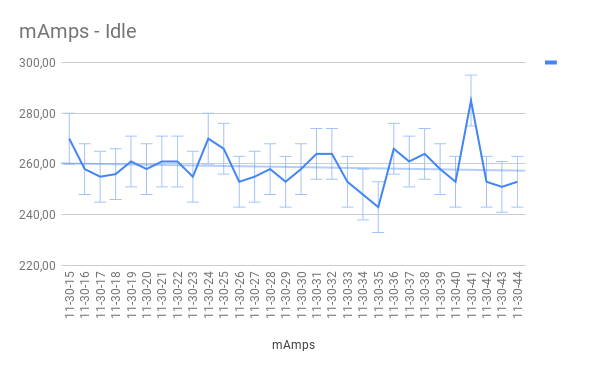
\includegraphics[width=.5\textwidth]{mAmps-idle.png}
\caption{Consumo em modo idle}
\label{fig:mamps_idle}
\end{figure}

\begin{figure}[ht]
\centering
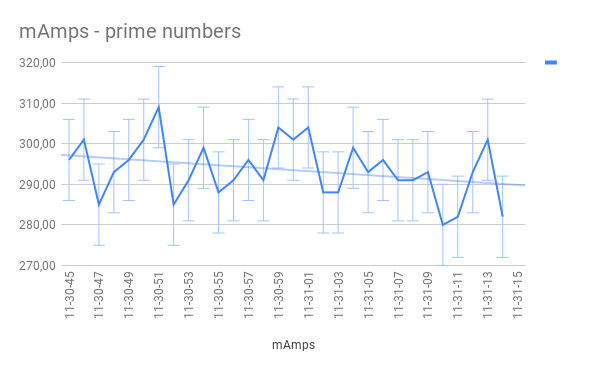
\includegraphics[width=.5\textwidth]{mAmps-full.png}
\caption{Consumo em modo full}
\label{fig:mamps_full}
\end{figure}

A simulação do uso de árvore Merkle ficou em torno de {\it 280mA} para inserção dos nós (figura \ref{fig:mamps_merkle_i}) e entre {\it 280mA} e {\it 290mA} a operação de diff (figura \ref{fig:mamps_merkle_q}).

\begin{figure}[ht]
\centering
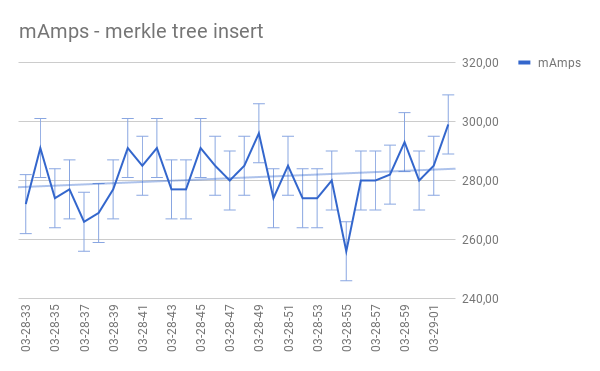
\includegraphics[width=.5\textwidth]{mAmps-merkle-insert.png}
\caption{Consumo Merkle insert}
\label{fig:mamps_merkle_i}
\end{figure}

\begin{figure}[ht]
\centering
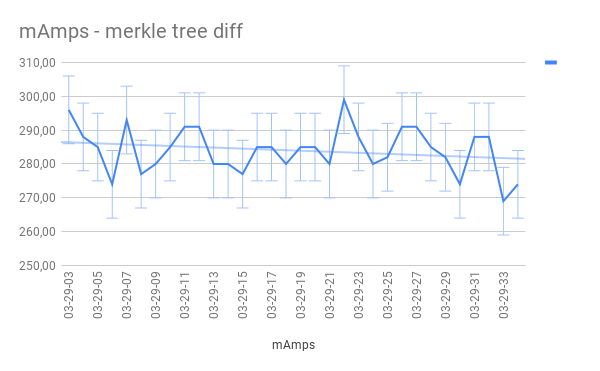
\includegraphics[width=.5\textwidth]{mAmps-merkle-diff.png}
\caption{Consumo Merkle query}
\label{fig:mamps_merkle_q}
\end{figure}

O consumo para as operações de autenticação de medições e operações utilizando {\it CRDT}'s apresentaram consumo entre {\it 280mA}-{\it 290mA} (figura \ref{fig:mamps_mac}) e {\it 285mA}-{\it 290mA} (figura \ref{fig:mamps_crdt}) respectivamente. A variação de consumo para o uso de {\it CRDT} consiste nas operações de {\it update} e {\it query}. A operação de {\it merge} para o {\it CRDT} utilizado consiste em acionar a operação de {\it update} para cada entrada do valor que deseja-se combinar, sendo assim, ela não foi medida separadamente.

\begin{figure}[ht]
\centering
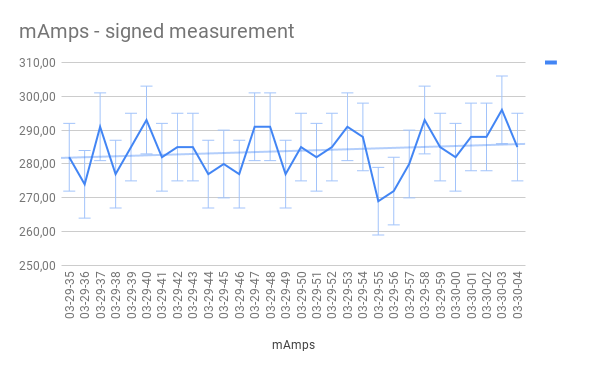
\includegraphics[width=.5\textwidth]{mAmps-mac.png}
\caption{Consumo autenticação de medições}
\label{fig:mamps_mac}
\end{figure}

\begin{figure}[ht]
\centering
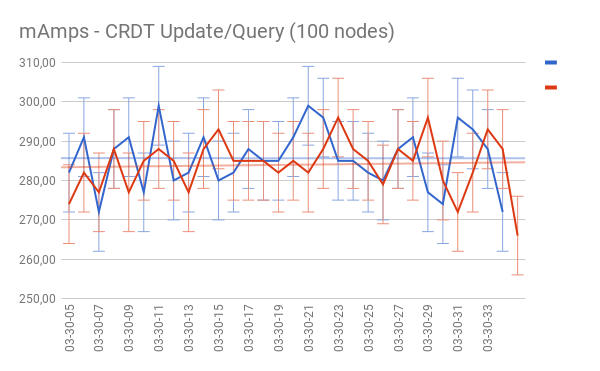
\includegraphics[width=.5\textwidth]{mAmps-crdt.png}
\caption{Consumo CRDT update (azul) / query (vermelho)}
\label{fig:mamps_crdt}
\end{figure}

\section{Conclusão}

Algumas aplicações precisam funcionar mesmo em ambientes onde não exista acesso a internet ou mesmo uma rede de dados estável. Nessas situações não é possível desenvolver assumindo que um servidor central é o responsável por garantir a consistência dos dados.

Nessas situações a utilização das estruturas apresentadas (Árvore Merkle e {\it CRDT}) permite que muitos dos problemas causados por sincronização de dados \ensuremath{P_{2}P} sejam resolvidos de maneira mais simples.

Tais estruturas afetam o consumo dos aparelhos, porém a alteração de {\it 30 a 40mA} não inviabiliza o uso das mesmas.

\section{Trabalhos futuros}

Os tipos {\it CRDT} são uma classe de estruturas de dados, \cite{shapiro:11} definem outras estruturas. Uma avaliação do custo computacional e de energia de outras estruturas pode ser feita. Além disso o algoritmo de hash da Árvore Merkle utilizado (SHA-1) pode ser substituido por outros mais recentes e com um tamanho maior (SHA-256, SHA-3).

Além disso, a medição por efeito {\it hall} não é tão precisa quanto a medição por resistor {\it shunt}. Porém o autor não possui acesso a equipamento para efetuar tal mediação, refazer as medições utilizando outra técnica ajuda a aumentar a confiança nos valores obtidos.

\bibliographystyle{sbc}
\bibliography{bibliografia}

\end{document}